\documentclass{beamer}

%Вариант 4

\usepackage[utf8]{inputenc}
\usepackage[russian]{babel}
\usepackage{ragged2e}
\usepackage{times}

\definecolor{darkgreen}{rgb}{0.0, 0.5, 0.0}

\begin{document}
\fontsize{9}{11}\selectfont


\begin{frame}[t]

\begin{figure}[h]

\frametitle{\begin{minipage}[b]{0.9\textwidth}
Мера количества информации по Шеннону
\end{minipage}
\hspace{0cm}
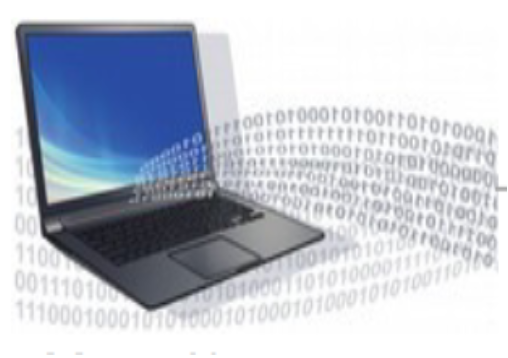
\includegraphics[width=0.15\textwidth, left]{логотип.png}}
\end{figure}
\vspace{-0.9cm}
\hline\\[0.1cm]


\begin{figure}[h]
\RaggedRight
\begin{minipage}[b]{0.8\textwidth}

 Мера хартли подходит лишь для систем с равновероятными состояниями. Если состояния системы S не равновероятны, используют меру Шеннона:
$$i(S) = -\sum_{i=1}p_{i} \cdot \log_{2}{p_{i}},$$

где N – число состояний системы,
pi – вероятность того, что система S находится в
состоянии i (сумма всех pi равна 1).
\end{minipage}

\RaggedLeft
\vspace{-4cm}
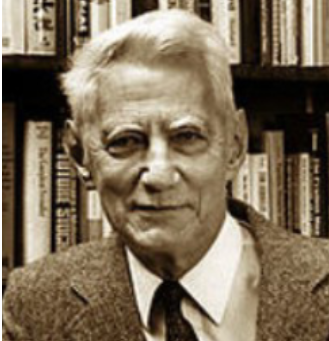
\includegraphics[width=0.2\textwidth]{Шеннон.png}\\
Клод Шеннон\\
(1916--2001)
\end{figure}
\vspace{0.5cm}

\begin{center}
\textbf{\textcolor{darkgreen}{Формула Хартли является частным случаем формулы Шеннона!}}
\end{center}

Пример 1. Количество информации в акте подбрасывания обычной монеты по формуле Хартли
равно $\log_{2}{p_{2}} = 1$ бит. По формуле Шеннона получим то же: $i_{s1} = -0,5*\log_{2}{0,5} - 0,5*\log_{2}{0,5} = 1$ бит.\\
Пример 2. При подбрасывании монеты со смещённым центром тяжести количество
непредсказуемости становится меньше:$i_{s2} = -0,75*\log_{2}{0,75} - 0,25*\log_{2}{0,25}\approx  0,8 $ бит.

\end{frame}

\begin{frame}[t]

\begin{figure}[h]

\frametitle{\begin{minipage}[b]{0.9\textwidth}
Пример использования меры Шеннона
\end{minipage}
\hspace{0cm}
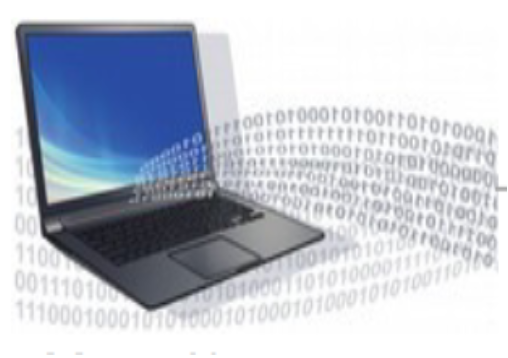
\includegraphics[width=0.15\textwidth, left]{логотип.png}}
\end{figure}
\vspace{-0.9cm}
\hline\\[0.3cm]
Шулер наугад вытаскивает одну карту из стопки, содержащей 9 известных ему карт: 3
джокера, 3 туза, 1 король, 1 дама и 1 валет. Какое количество информации для шулера
содержится в этом событии s?\\
\begin{center}
Вероятность вытащить \begin{Bmatrix}
    \\\text{джокера}
    \\\text{туза}
    \\\text{короля}
    \\\text{даму}
    \\\text{валета}
\end{Bmatrix} 
равна \begin{Bmatrix}

    \\3/9 = 1/3
    \\3/9 = 1/3
    \\1/3
    \\1/3
    \\1/3
\end{Bmatrix} 
\end{center}
Количество информации, выраженное в тритах, равно:
$$-(\frac{1}{3} \cdot\log_{3}{\frac{1}{3}} + \frac{1}{3} \cdot\log_{3}{\frac{1}{3}} + \frac{1}{9} \cdot\log_{3}{\frac{1}{9}} + \frac{1}{9} \cdot\log_{3}{\frac{1}{9}} + \frac{1}{9} \cdot\log_{3}{\frac{1}{9}})=$$\\ 
$$=\frac{1}{3}+ \frac{1}{3}+ \frac{1}{9}+ \frac{1}{9}+ \frac{1}{9}=1\frac{1}{3}\approx \log_{3}{14}$$
\end{frame}
\begin{frame}[t]

\begin{figure}[h]

\frametitle{\begin{minipage}[b]{0.9\textwidth}
Нестрогий вывод формулы Шеннона
\end{minipage}
\hspace{0cm}
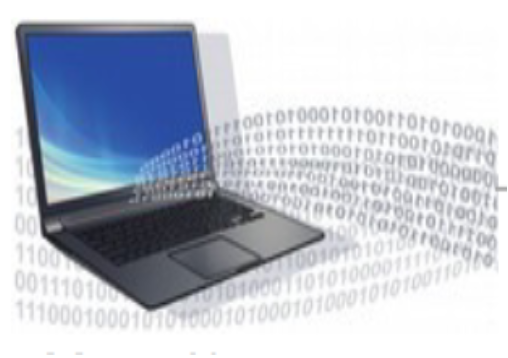
\includegraphics[width=0.15\textwidth, left]{логотип.png}}
\end{figure}
\vspace{-0.9cm}
\hline\\[0.3cm]
\textcolor{darkgreen}{Задача}
Монета имеет смещённый центр тяжести. Вероятность выпадения «орла» – 0,25,
вероятность выпадения «решки» – 0,75. Какое количество информации содержится в одном
подбрасывании?\\
\vspace{0.5cm}
\textcolor{darkgreen}{Решение}\\

\begin{itemize}
\item Пусть монета была подброшена N раз $(N→\infty)$, из которых «решка» выпала M раз, «орёл» —
K раз (очевидно, что N = M + K).
\item Количество информации в N подбрасываниях: $i_{N}$ = M*i(«решка») + K*i(«орёл»).
\item Тогда среднее количество информации в одном подбрасывании:\\
$i_{1}=i_{N}/N$ = (M/N)*i(«решка»)+(K/N)*i(«орёл») = p(«решка»)*i(«решка»)+p(«орёл»)*i(«орёл»)
\item Подставив формулу Шеннона для i, окончательно получим:\\
$i_{1}=-p(\text{«решка»})*\log_{x}{p}(\text{«решка»})-p(\text{«орел»})*\log_{x}{p}(\text{«орел»})\approx$ 0,8 бит.
\end{itemize}


\end{frame}
\begin{frame}[t]

\begin{figure}[h]

\frametitle{\begin{minipage}[b]{0.9\textwidth}
Приставки для единиц измерения
количества информации/данных: проблема
\end{minipage}
\hspace{0cm}
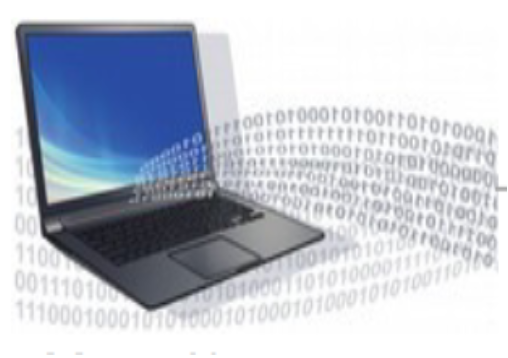
\includegraphics[width=0.15\textwidth, left]{логотип.png}}
\end{figure}
\vspace{-0.9cm}
\hline\\[1cm]

\begin{figure}[h]

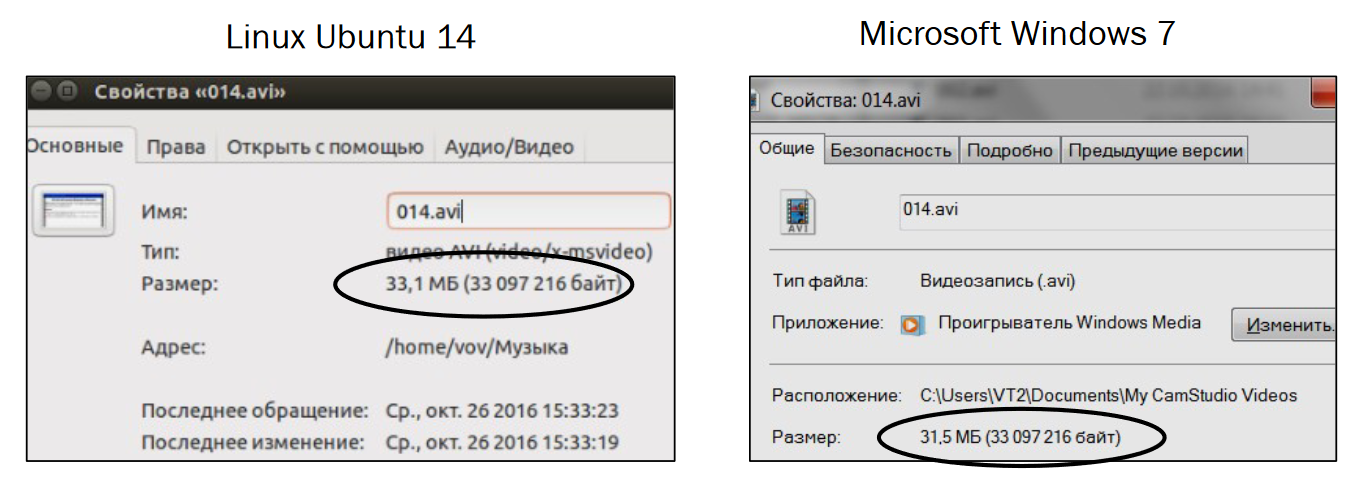
\includegraphics[width=1\textwidth,]{слайд20.png}
\end{figure}

\begin{center}
    33 097 216 байт — это \textcolor{darkgreen}{33,1}
    МБ или 
    \textcolor{darkgreen}{31,5} 
    МБ?
\end{center}
\end{frame}

\begin{frame}[t]

\begin{figure}[h]

\frametitle{\begin{minipage}[b]{0.9\textwidth}
Приставки для единиц измерения
количества информации/данных: решение
\end{minipage}
\hspace{0cm}
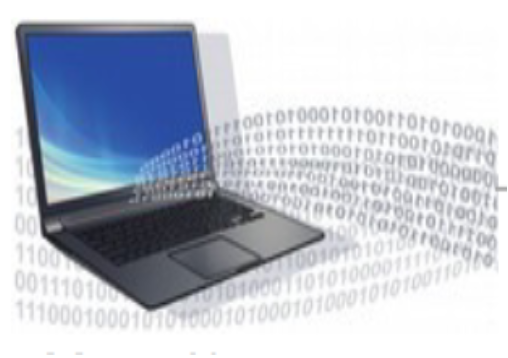
\includegraphics[width=0.15\textwidth, left]{логотип.png}}
\end{figure}
\vspace{-0.9cm}
\hline\\[0.3cm]
1. \textcolor{darkgreen}{IEEE 1541-2002}
– Институт инженеров по электротехнике и радиоэлектронике.\\
2. \textcolor{darkgreen}{ISO/IEC 80000-13:2008}
– Международная организация по стандартизации.\\
3. \textcolor{darkgreen}{ГОСТ IEC 60027-2-2015} – Международная электротехническая комиссия.

\begin{figure}[h]

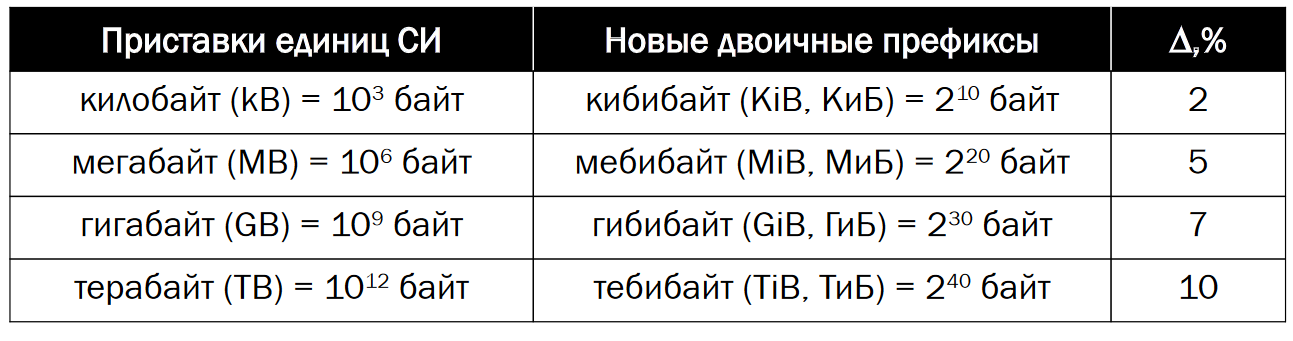
\includegraphics[width=0.9\textwidth,]{слайд21.png}
\end{figure}

\textcolor{darkgreen}{Краткое обозначение битов и байтов:} 
\RaggedLeft
b = bit = бит, B = Б = байт
1024 B = 1024 Б = 8192 b = 8192 бит = 8 Кибит = 1 КиБ = 1 KiB
\end{frame}


\end{document}




